\newpage
\solutions{Grafy 2}

\begin{problem}{1}
	W pewnej grupie $2n$ osób, gdzie $n$ jest liczbą całkowitą nie mniejszą od $2$, każda osoba zna co najmniej $n$ innych osób. Wykazać, że możemy usadzić pewne cztery osoby przy okrągłym stole, aby każda z nich znała swoich sąsiadów.
\end{problem}

\noindent
Jeśli wszystkie osoby by się znały, to dowolna cztery z nich spełniają warunki zadania. Załóżmy, że są dwie osoby -- $A$ i $B$, które się nie znają. Każda z nich zna co najmniej $n$~osób spośród pozostałych $2n - 2$ osób. Stąd są co najmniej dwie osoby, które są znane zarówno przez $A$, jak i przez $B$. Nazwijmy je $C$ i $D$. Wówczas ustawienie $A$, $C$, $B$, $D$ spełnia warunki zadania. 

\vspace{5px}

\begin{problem}{2}
	Dana jest pewna dodatnia liczba całkowita $k$ oraz pewna liczba chłopców i dziewczyn. Każda z osób zna dokładnie $k$ osób płci przeciwnej. Wykazać, że można zaaranżować pary między chłopcami i dziewczynami, tak, aby każda osoba była w dokładnie jednej parze.
\end{problem}

\noindent
Wykażemy, że spełniony jest warunek Halla. Załóżmy nie wprost, że istnieje podzbiór $t$~dziewczyn, że znają one łącznie mniej niż $t$~chłopców. Skoro każda dziewczyna zna dokładnie $k$~chłopców, to znajomości damsko-męskich, dla których dziewczyna należy do rozpatrywanego podzbioru jest dokładnie~$tk$. Skoro każdy chłopiec na dokładnie $k$~dziewczyn, to musi znać co najwyżej~$k$ dziewczyn z rozpatrywanego zbioru. Skoro chłopców, którzy znają co najmniej jedną z nich jest co najwyżej $t - 1$, to łączna liczba tych znajomości jest nie większa niż $k(t - 1)$. Daje to sprzeczność.

\vspace{5px}

\begin{problem}{3}
	Dany jest graf, w którym każdy wierzchołek ma stopień co najwyżej $100$. Zbiór krawędzi nazwiemy \textit{idealnym}, jeśli żadne dwie krawędzie należące do niego nie mają wspólnego końca oraz nie da się dołożyć żadnej krawędzi, aby ta własność była zachowana. W każdym ruchu usunięto dowolny  idealny zbiór krawędzi, które przed wykonaniem tego ruchu należały do rozpatrywanego grafu. Wykazać, że po wykonaniu dowolnych $199$ ruchów, graf nie będzie zawierał żadnej krawędzi.
\end{problem}

\noindent
Rozpatrzmy dowolną krawędź -- przyjmijmy, że jest ona między wierzchołkami $u$ i $v$. Wykażemy, że po wykonaniu dowolnych $198$ ruchów zostanie ona usunięta. Analogicznie rozumując dla każdej krawędzi udowodnimy tezę.

\vspace{5px}
\noindent
Załóżmy, że pewien zbiór idealny nie zawiera krawędzi pomiędzy $u$ i $v$. Jeśli ten zbiór nie zawierałby żadnej krawędzi wychodzącej z $u$ albo $v$, to możnaby do niego dołożyć krawędź pomiędzy $u$ i $v$, co daje sprzeczność z maksymalnością tego zbioru. 

\vspace{5px}
\noindent
Pozostałych wychodzących z jednego z~wierzchołków $u$ lub $v$ jest co najwyżej $2 \cdot 99 = 198$. W takim razie w ciągu $199$ ruchów istnieje taki ruch, w~którym nie usuniemy jednej z~nich. Z wyżej wykazanego wniosku wynika, że usuniemy wówczas krawędź pomiędzy~$u$~i~$v$.

\begin{problem}{4}
	Dany jest graf planarny, w którym $e$ to liczba krawędzi, a $v \geqslant 3$ to liczba wierzchołków. Wykazać, że zachodzi nierówność
	\[
		e \leqslant 3v - 6.
	\]
\end{problem}

\noindent
Skoro każda ściana ma co najmniej $3$ boki, to dodając liczbę boków każdej ze ścian otrzymamy liczbę nie mniejszą niż $3f$. Jest to dwukrotność liczby boków, bo każdy bok należy do dwóch ścian. Stąd ta liczba jest równa $2e$. Mamy więc
\[
	2e \geqslant 3f.
\]
Na mocy twierdzenia Eulera mamy
\begin{align*}
	v - e + f &= 1 + c \geqslant 2, \\
	v - 2 &\geqslant e - f, \\
	3v  - 6 &\geqslant 3e - 3f \geqslant e.
\end{align*}

\begin{problem}{5}
	Na pewnym przyjęciu okazało się, że każdy zna co najmniej $k$ innych gości, gdzie $k \geqslant 2$ jest pewną liczbą naturalną. Wykazać, że istnieje taka liczba naturalna $n\geqslant k + 1$, że można usadzić pewnych $n$ uczestników przyjęcia przy okrągłym stole tak, aby każdy znał obu swoich sąsiadów.
\end{problem}

\noindent
Rozpatrzmy graf, w którym goście są wierzchołkami, a znajomości krawędziami.
Weźmy ścieżkę o maksymalnej długości w rozpatrywanym grafie. Niech $a$ będzie jednym z jej skrajnych wierzchołków, a kolejne wierzchołki oznaczmy jako $a_1,\; a_2,\; ...,\; a_t$. Jeśli $a$ byłby połączony z pewnym wierzchołkiem spoza analizowanej ścieżki, to można by ten wierzchołek do tej ścieżki dołożyć, wydłużając ją. Przeczyłoby to jednak jej maksymalności.

\begin{center}
	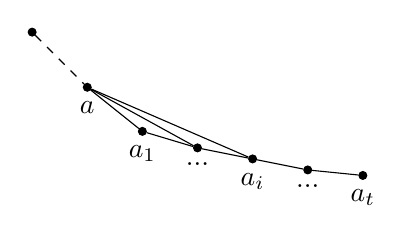
\begin{tikzpicture}[scale=0.7]
		\tikzset{vertex/.style = {shape=circle,draw, inner sep = 1pt, fill=black}}

		\node[vertex] (A) at (0,4) {};
		\node[vertex, label=below:$a$] (B_1) at (1,3) {};
		\node[vertex, label=below:$a_1$] (B_2) at (2,2.2) {};
		\node[vertex, label=below:$...$] (B_3) at (3,1.9) {};
		\node[vertex, label=below:$a_i$] (B_4) at (4,1.7) {};
		\node[vertex, label=below:$...$] (B_5) at (5,1.5) {};
		\node[vertex, label=below:$a_t$] (B_6) at (6,1.4) {};


		\draw[dashed] (A)--(B_1);
		\draw (B_1)--(B_3);
		\draw (B_1)--(B_4);
		\draw (B_1)--(B_2);
		\draw (B_2)--(B_3);
		\draw (B_3)--(B_4);
		\draw (B_4)--(B_5);
		\draw (B_5)--(B_6);

	\end{tikzpicture}
\end{center}

\noindent
Z $a$ wychodzi co najmniej $k$ krawędzi, każda z nich łączy go z jednym wierzchołkiem spośród $a_1,\; a_2,\; ...,\; a_t$. Niech $a_i$ będzie wierzchołkiem połączonym z $a$, dla którego $i$ jest maksymalne. Wiemy, że spośród $a_1,\; a_2,\; ...,\; a_{i - 1}$ co najmniej $k - 1$ jest połączonych z $a$, stąd
\begin{align*}
	i - 1 \geqslant k - 1, \\
	i + 1 \geqslant k + 1.
\end{align*}
Usadzając przy stole osoby 
\[
	a, a_1,\; a_2,\; ...,\; a_{i - 1}, \; a_i
\]
otrzymujemy tezę.

\begin{problem}{6}
	Krawędzi grafu pełnego o $n \geqslant 3$ wierzchołkach zostały pokolorowane w taki sposób, że każdy kolor został użyty do pokolorowania co najwyżej $n - 2$ krawędzi. Wykazać, że istnieje podgraf tego grafu, będący trójkątem, o krawędziach parami różnych kolorów.
\end{problem}

\noindent
Przeprowadźmy rozumowanie nie wprost -- zakładamy, że żaden trójkąt nie jest różnokolorowy. Rozpatrzmy taki kolor $c$ i taki zbiór wierzchołków $A$, że pomiędzy każdymi dwoma wierzchołkami w $A$ istnieje ścieżka złożona z krawędzi koloru $c$. Przyjmijmy dodatkowo, że $A$ jest maksymalnym zbiorem o tej własności.

\vspace{10px}
\noindent
Załóżmy, że istnieje pewien wierzchołek $v$ w tym grafie, który nie należy do zbioru $A$. Niech $a$ oznacza pewien wierzchołek z $A$, zaś $b \in A$ niech będzie sąsiadem $a$, o ile takowy istnieje. Zauważmy, że krawędzie $va$ i $vb$ nie mogą być koloru $c$, bo wówczas moglibyśmy dorzucić wierzchołek $v$ do $A$. Tak być nie może, bo $A$ jest maksymalnym zbiorem o~postulowanej własności. 
\begin{center}
	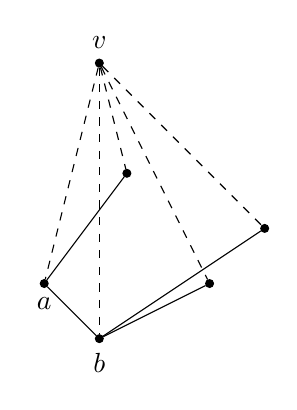
\begin{tikzpicture}[scale=0.7]
		\tikzset{vertex/.style = {shape=circle,draw, inner sep = 1pt, fill=black}}

		\node[vertex, label=above:$v$] (A) at (0,4) {};

		\node[vertex, label=below:$a$] (B_1) at (-1,0) {};
		\node[vertex, label=below:$b$] (B_2) at (0,-1) {};
		\node[vertex] (B_3) at (2,0) {};
		\node[vertex] (B_4) at (3,1) {};
		\node[vertex] (B_5) at (0.5,2) {};




		\draw[dashed] (A)--(B_1);
		\draw[dashed] (A)--(B_2);
		\draw[dashed] (A)--(B_3);
		\draw[dashed] (A)--(B_4);
		\draw[dashed] (A)--(B_5);

		\draw (B_1)--(B_2);
		\draw (B_1)--(B_5);
		\draw (B_2)--(B_3);
		\draw (B_2)--(B_4);

	\end{tikzpicture}
\end{center}

\vspace{10px}
\noindent
Niech krawędź $va$ ma kolor $c_1$. Skoro trójkąt $vab$ nie może być różnokolorowy, krawędź $vb$ ma również kolor $c_1$. Stąd wszystkie krawędzie z $v$ do sąsiadów $a$ są koloru $c_1$. Analogicznie wszystkie krawędzie z $v$ do sąsiadów sąsiadów wierzchołka $a$ są koloru $c_1$. Przeprowadzając to rozumowanie dalej otrzymujemy, że wszystkie wierzchołki ze zbioru $A$ są połączone z~wierzchołkiem~$v$ krawędzią koloru~$c_1$. Zbiór wierzchołków $A \cup v$ oraz kolor $c_1$ mają własność, co do której zakładaliśmy, że maksymalnym zbiorem ją posiadającym jest $A$. Ta sprzeczność dowodzi tego, że nie może istnieć wierzchołek $v$, czyli zbiór $A$ jest pełnym zbiorem wierzchołków.

\vspace{10px}
\noindent
Rozpatrzmy graf składający się tylko z krawędzi koloru $c$. Jest to graf spójny o $n$ wierzchołkach. Musi mieć on więc co najmniej $n - 1$ krawędzi. Przeczy to założeniu zadania, że jest ich co najmniej $n - 2$.
\vspace{10px}

\begin{remark}
	Dowód faktu, że graf spójny o $n$ wierzchołkach musi mieć co najmniej $n - 1$ krawędzi pozostawiamy czytelniczce/czytelnikowi jako ćwiczenie.
\end{remark}
